\documentclass{standalone}
\usepackage[utf8]{inputenc}
\usepackage[T1]{fontenc}
\usepackage{graphicx}
\usepackage{amsmath}
\usepackage[]{pgf,tikz}
\usepackage[]{circuitikz}
\usetikzlibrary{arrows,shapes,calc,positioning}


\newcommand{\valve}{%
% A clipped circle is drawn
    \draw (0.3,0) arc (0:180:0.3) -- cycle;
    \draw (0,0) -- (0,-0.3);
    \draw (-0.3, -0.15) -- (0.3, -0.45) -- (0.3, -0.15) -- (-0.3, -0.45) -- cycle;
}

\begin{document}
\begin{tikzpicture}
  \node[] (tank) {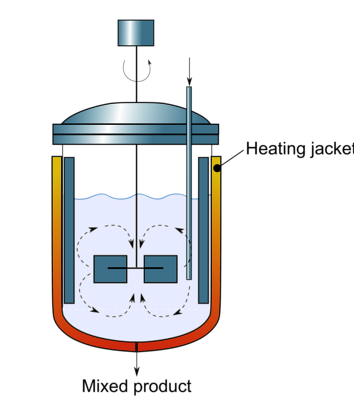
\includegraphics[width=6cm]{./Agitated_vessel_heated_simple}};

%  \draw[help lines,xstep=.1,ystep=.1] (-0,-0) grid (3,4);
%\foreach \x in {0,1,...,9} { \node [anchor=north] at (\x/10,0) {0.\x}; }
%\foreach \y in {0,1,...,9} { \node [anchor=east] at (0,\y/10) {0.\y}; }

\node[] (T) at (-1, 0) {$c$};
\node[circle,  left of=T, node distance=30mm,] (TT) {\sf };
\node[circle,  below of=tank, node distance=50mm,] (TT1) {\sf };
\node[circle, draw,  left of=TT1, node distance=8mm, minimum height=8mm] (TT2) {\sf };
\node[circle, draw, left of=TT2, node distance=47.4mm,] (TC) {\sf TC};
\node[coordinate, above of=TC, node distance=22mm] (vlv) {};

\coordinate (vlvdraw) at ($(vlv.north) + (0cm, -0.6cm)$);
\coordinate (vlvcontr) at ($(vlv.north) + (0cm, -0.9cm)$);
\coordinate (vlvin) at ($(vlv.west) + (-0.3cm, -0.32cm)$);
\coordinate (vlvout) at ($(vlv.east) + (0.3cm, -0.32cm)$);

\begin{scope}[shift=(vlvdraw), rotate=180] 
  \valve
\end{scope}



\draw[double, thick, double distance=4pt] ($(tank) - (0.7,2.1)$) -- ++(0,-1cm) arc (180:270:1cm) -- node[pos=0,coordinate] (sensor) {} node[pos=0.1] {$c$}  ++(2.7, 0);
\draw[double, thick, double distance=4pt] ($(vlvin) - (2,0)$) -- (vlvin);
\draw[double, thick, double distance=4pt,] (vlvout) -- ++(2.7,0) ++(0,0) arc (-90:-10:1cm) ++(1.7,0) arc (190:270:1cm) -- ++(17mm, 0);
\draw[thin, ->] (vlvout) ++(1, 0) -- node[above] {\Large $u_v$} ++(1,0);

\draw[] (sensor) to[short, *-,] (TT2.east);
\draw[dashed, ->] (TT2.west) to (TC.east);

\draw[->] (TC) -- (vlvcontr);

\node at (0.7,2.7) {$Q$, $T_i, c_{i}$};

\end{tikzpicture}
\end{document}
